\documentclass[tikz,border=8pt]{standalone}
% Shared look for every TikZ diagram. Load with \input{../../tools/tikz-style.tex}
\usepackage[sfdefault]{roboto}
\usetikzlibrary{arrows.meta, positioning, shapes.geometric, calc, fit, backgrounds}
\definecolor{cblue}{HTML}{4C78A8}
\definecolor{corange}{HTML}{F58518}
\definecolor{cgreen}{HTML}{54A24B}
\definecolor{cred}{HTML}{E45756}
\definecolor{cpurple}{HTML}{B279A2}
\definecolor{cgrey}{HTML}{6B6B6B}
\tikzset{
  every picture/.style={font=\sffamily, line width=1.2pt},
  box/.style={draw=#1, fill=#1!12, rounded corners=4pt, align=center, inner sep=7pt, minimum height=1.1cm},
  box/.default=cgrey,
  arrow/.style={-{Stealth[length=3mm]}, draw=cgrey, line width=1.4pt},
  title/.style={font=\sffamily\bfseries\Large},
  note/.style={font=\sffamily\small, text=cgrey, align=center},
}
\AtBeginDocument{\hyphenpenalty=10000 \exhyphenpenalty=10000}

% Near the North Pole, seen from above (not to scale). Walking 1 m east along the circle 10 m from the pole changes
% the longitude by 1/10 rad = 5.7 degrees; 1 m along the circle 1 m from the pole changes it by 1 rad = 57.3 degrees.
% At the pole itself the longitude has no value: a singularity of latitude-longitude coordinates.
\begin{document}
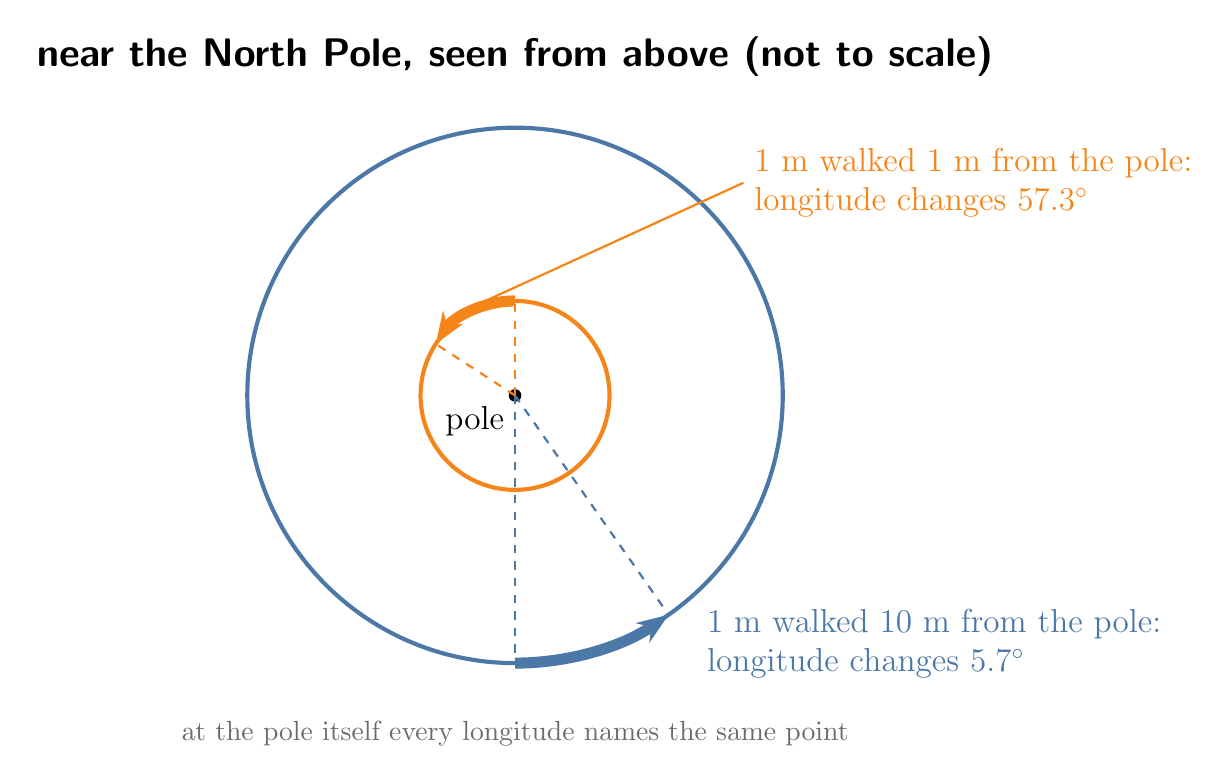
\begin{tikzpicture}[every node/.append style={font=\large}]
  \node[title] at (0,4.3) {near the North Pole, seen from above (not to scale)};
  \fill[black] (0,0) circle (0.08);
  \node[below left] at (0,0) {pole};
  % circle 10 m from the pole
  \draw[cblue, line width=1.5pt] (0,0) circle (3.4);
  \draw[cblue, line width=4pt, -{Stealth[length=4mm]}] (-90:3.4) arc (-90:-55:3.4);
  \draw[cblue, dashed, line width=0.8pt] (0,0) -- (-90:3.4);
  \draw[cblue, dashed, line width=0.8pt] (0,0) -- (-55:3.4);
  \node[cblue, align=left, anchor=west] at (2.3,-3.15) {1 m walked 10 m from the pole:\\ longitude changes 5.7$^\circ$};
  % circle 1 m from the pole
  \draw[corange, line width=1.5pt] (0,0) circle (1.2);
  \draw[corange, line width=4pt, -{Stealth[length=4mm]}] (90:1.2) arc (90:147:1.2);
  \draw[corange, dashed, line width=0.8pt] (0,0) -- (90:1.2);
  \draw[corange, dashed, line width=0.8pt] (0,0) -- (147:1.2);
  \node[corange, align=left, anchor=west] (ol) at (2.9,2.7) {1 m walked 1 m from the pole:\\ longitude changes 57.3$^\circ$};
  \draw[corange, line width=0.8pt] (ol.west) -- (118:1.25);
  \node[note, font=\normalsize, align=center] at (0,-4.3) {at the pole itself every longitude names the same point};
\end{tikzpicture}
\end{document}
